\documentclass[11pt,a4paper]{article}

\usepackage[utf8]{inputenc}
\usepackage[margin=2.5cm]{geometry}
\usepackage{amsmath,amssymb,amsthm}
\usepackage{booktabs,array}
\usepackage{enumitem}
\usepackage[most]{tcolorbox}
\usepackage{tikz}
\usetikzlibrary{arrows.meta,calc,decorations.markings,angles,quotes,positioning}
\usepackage{pgfplots}
\pgfplotsset{compat=1.16}
\usepackage[colorlinks=true,linkcolor=blue!50!black,urlcolor=blue!50!black]{hyperref}

% ---------- macros ----------
\newcommand{\R}{\mathbb{R}}
\newcommand{\W}{\mathcal{W}}
\newcommand{\C}{\mathcal{C}}
\newcommand{\SO}{\mathrm{SO}}
\newcommand{\SE}{\mathrm{SE}}
\newcommand{\Sph}{\mathbb{S}}
\newcommand{\norm}[1]{\lVert #1\rVert}
\newcommand{\pts}[1]{\emph{(notes p.~#1)}}

% ---------- theorem environments ----------
\theoremstyle{definition}
\newtheorem{definition}{Definition}[section]
\newtheorem{example}[definition]{Example}
\newtheorem{algorithm}[definition]{Algorithm}
\theoremstyle{plain}
\newtheorem{lemma}[definition]{Lemma}
\newtheorem{proposition}[definition]{Proposition}
\newtheorem{theorem}[definition]{Theorem}
\newtheorem{corollary}[definition]{Corollary}

\tcbset{
  thmbox/.style={enhanced,breakable,colback=gray!4,colframe=gray!60!black,
    boxrule=0.6pt,arc=2pt,left=6pt,right=6pt,top=4pt,bottom=4pt}
}
% boxed versions of the amsthm environments
\tcolorboxenvironment{definition}{thmbox}
\tcolorboxenvironment{example}{thmbox}
\tcolorboxenvironment{algorithm}{thmbox}
\tcolorboxenvironment{lemma}{thmbox}
\tcolorboxenvironment{proposition}{thmbox}
\tcolorboxenvironment{theorem}{thmbox}
\tcolorboxenvironment{corollary}{thmbox}

% blue intuition box
\newtcolorbox{intuition}{enhanced,breakable,colback=blue!5,colframe=blue!55!black,
  fonttitle=\bfseries,title={Intuition},boxrule=0.6pt,arc=2pt,
  left=6pt,right=6pt,top=3pt,bottom=3pt}

\title{\textbf{Configuration Space}\\[2pt]\large Lecture notes -- Autonomous \& Mobile Robotics, Lecture 1}
\author{}
\date{}

\begin{document}
\maketitle
\tableofcontents
\bigskip


% =====================================================================
\section{Configuration Space and Workspace}\pts{1--2}
% =====================================================================

\subsection{The idea}

The central idea is to \emph{define a suitable space in which the robot is a single point}. Once the robot is a point, two core tasks become much simpler to formulate:
\begin{itemize}[nosep]
  \item \textbf{planning} (find a path for the point from a start to a goal),
  \item \textbf{control} (make the point follow that path).
\end{itemize}
(Fun fact from the notes: the C-space concept was born to do \emph{collision avoidance}.)

\begin{intuition}
Think of a huge, awkwardly shaped sofa that has to be moved through a door. Reasoning about every corner of the sofa at the same time is painful. If instead we find a space where the whole sofa is \emph{one dot}, and the ``forbidden'' places for the dot are exactly the sofa positions that hit a wall, then moving the sofa becomes moving a dot around obstacles.
\end{intuition}

\subsection{Robots and workspaces}

\begin{definition}[Robot and workspace]
A \emph{robot} is a collection of $n_b$ rigid bodies (we assume rigid robots) moving in a \emph{workspace} $\W=\R^2$ or $\W=\R^3$, the physical space in which the robot moves.
\begin{itemize}[nosep]
  \item If $\W=\R^2$ the robot is \emph{planar}; if $\W=\R^3$ it is \emph{spatial}.
  \item If $n_b=1$ the robot is \emph{single-body}; if $n_b>1$ it is \emph{multi-body}.
\end{itemize}
\end{definition}

\begin{example}
A car can be modelled as a single body, whereas a car with a trailer is a multi-body system ($n_b=2$).
\end{example}

\subsection{Configuration and generalized coordinates}

\begin{definition}[Posture and configuration]
The \emph{posture} of a robot is the position of all its points in $\W$. A \emph{configuration} is a \emph{minimal} set of parameters that defines the posture of the robot in $\W$. The corresponding vector
\[
  q=\begin{pmatrix} q_1\\ \vdots\\ q_n\end{pmatrix}
\]
is called a \emph{configuration vector}, and each $q_i$ is a \emph{generalized coordinate}.
\end{definition}

The generalized coordinates are of two kinds:
\begin{itemize}[nosep]
  \item \textbf{Cartesian coordinates}: identify the position of representative points of the robot; they take values in $\R^2$ or $\R^3$.
  \item \textbf{Angular coordinates}: identify the orientation of the bodies of the robot; they take values in $\SO(2)$ (planar: one parameter) or $\SO(3)$ (spatial: three parameters).
\end{itemize}


\begin{figure}[ht]
\centering
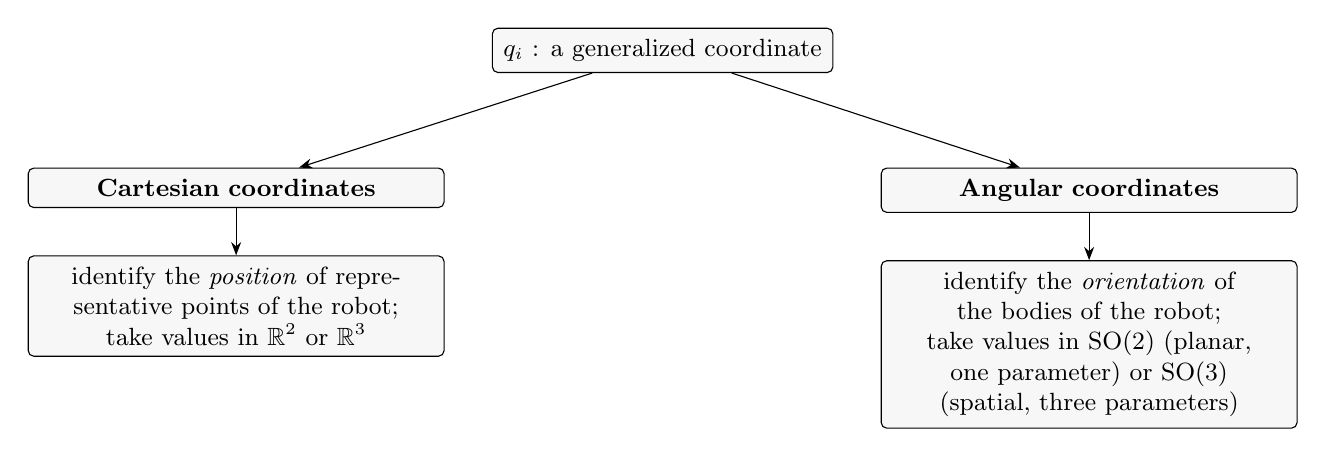
\begin{tikzpicture}[>=Stealth,node distance=8mm,
  box/.style={draw,rounded corners=2pt,fill=gray!6,align=center,inner sep=4pt,font=\small}]
  \node[box] (q) {$q_i$ : a generalized coordinate};
  \node[box,below left=12mm and 6mm of q,text width=5cm] (c) {\textbf{Cartesian coordinates}};
  \node[box,below right=12mm and 6mm of q,text width=5cm] (a) {\textbf{Angular coordinates}};
  \node[box,below=6mm of c,text width=5cm] (c2) {identify the \emph{position} of representative points of the robot;\\ take values in $\R^2$ or $\R^3$};
  \node[box,below=6mm of a,text width=5cm] (a2) {identify the \emph{orientation} of the bodies of the robot;\\ take values in $\SO(2)$ (planar, one parameter) or $\SO(3)$ (spatial, three parameters)};
  \draw[->] (q) -- (c); \draw[->] (q) -- (a);
  \draw[->] (c) -- (c2); \draw[->] (a) -- (a2);
\end{tikzpicture}
\caption{The two kinds of generalized coordinates.}
\end{figure}

\begin{intuition}
``Minimal'' is the key word. The posture is the full, redundant description (every point of every body); the configuration is the shortest list of numbers from which the posture can be reconstructed. A rigid rectangle in the plane has infinitely many points, but three numbers $(x,y,\theta)$ tell you where all of them are.
\end{intuition}

\subsection{Configuration space}

\begin{definition}[Configuration space]
The \emph{configuration space} (C-space) $\C$ of a robot is the set of all possible values of $q$. Its dimension $n=\dim\C$ is the number of degrees of freedom of the robot.
\end{definition}

\begin{intuition}
The C-space is the ``catalogue of all poses the robot can be in''. Each point of $\C$ \emph{is} one pose. A curve in $\C$ is therefore a motion of the robot in the physical space, which is exactly why planning for a robot reduces to planning for a point.
\end{intuition}

% =====================================================================
\section{Examples of Configuration Spaces}\pts{2--3}
% =====================================================================

\begin{example}[Point robot in $\W=\R^3$]
$q=(x,y,z)^\top$, so $\C=\R^3=\W$ and $n=3$.
\end{example}

\begin{example}[Disk robot in $\W=\R^2$]
Since a disk looks the same under any rotation, its orientation is irrelevant: $q=(x,y)^\top$, $\C=\R^2=\W$, $n=2$.
\end{example}

\begin{figure}[ht]
\centering
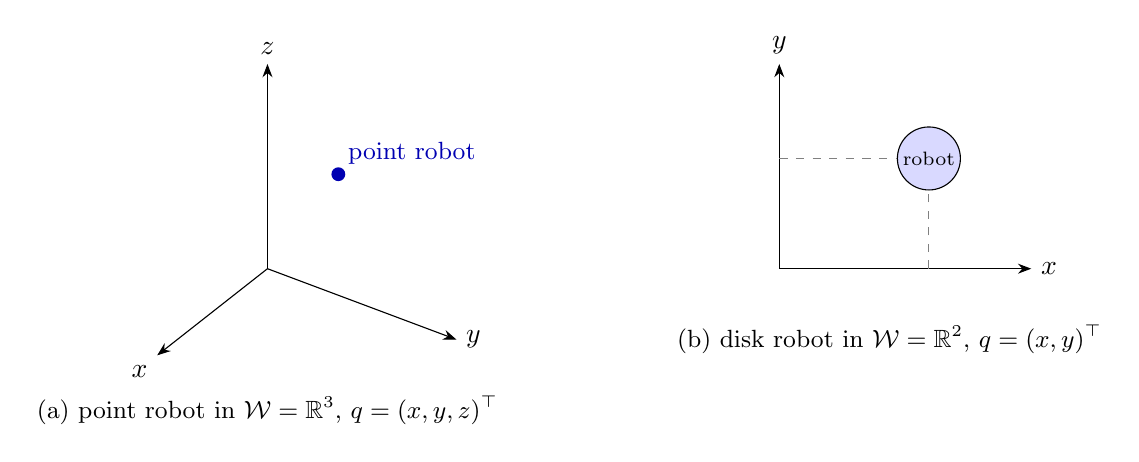
\begin{tikzpicture}[>=Stealth]
  % point robot in R^3
  \begin{scope}
    \draw[->] (0,0) -- (0,2.6) node[above] {$z$};
    \draw[->] (0,0) -- (2.4,-0.9) node[right] {$y$};
    \draw[->] (0,0) -- (-1.4,-1.1) node[below left] {$x$};
    \fill[blue!70!black] (0.9,1.2) circle (2.5pt) node[above right] {\small point robot};
    \node at (0,-1.8) {\small (a) point robot in $\W=\R^3$, $q=(x,y,z)^\top$};
  \end{scope}
  % disk robot in R^2
  \begin{scope}[shift={(6.5,0)}]
    \draw[->] (0,0) -- (3.2,0) node[right] {$x$};
    \draw[->] (0,0) -- (0,2.6) node[above] {$y$};
    \draw[fill=blue!15] (1.9,1.4) circle (0.4);
    \node at (1.9,1.4) {\scriptsize robot};
    \draw[dashed,gray] (0,1.4) -- (1.5,1.4);
    \draw[dashed,gray] (1.9,0) -- (1.9,1.0);
    \node at (1.4,-0.9) {\small (b) disk robot in $\W=\R^2$, $q=(x,y)^\top$};
  \end{scope}
\end{tikzpicture}
\caption{Point robot and disk robot: in both cases $\C=\W$.}
\end{figure}

In both examples $\C$ and $\W$ coincide. A case where they differ:

\begin{example}[Disk with a tick]
We add a small mark (a ``tick'') to the disk, so that its orientation now matters. Then
\[
  q=\begin{pmatrix}x\\y\\\varphi\end{pmatrix},\qquad
  \C=\R^2\times \SO(2),\qquad n=3 ,
\]
where $\times$ is the Cartesian product.
\end{example}

\begin{figure}[ht]
\centering
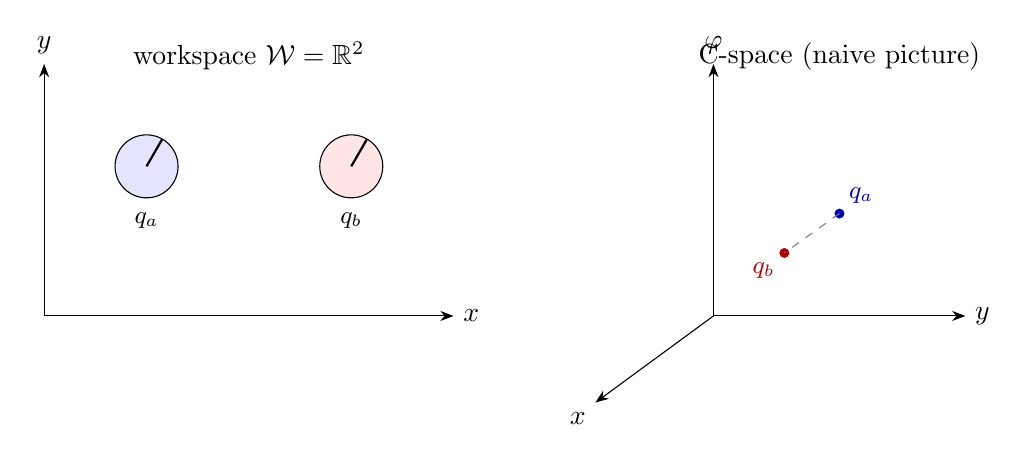
\begin{tikzpicture}[scale=1,>=Stealth]
% ---- workspace ----
\begin{scope}
  \draw[->] (0,0) -- (5.2,0) node[right] {$x$};
  \draw[->] (0,0) -- (0,3.2) node[above] {$y$};
  \node at (2.6,3.3) {workspace $\W=\R^2$};
  % configuration a
  \begin{scope}[shift={(1.3,1.9)}]
    \draw[fill=blue!10] (0,0) circle (0.4);
    \draw[thick] (0,0) -- (60:0.4);
    \node[below=2pt] at (0,-0.4) {\small $q_a$};
  \end{scope}
  % configuration b: same y and phi, different x
  \begin{scope}[shift={(3.9,1.9)}]
    \draw[fill=red!10] (0,0) circle (0.4);
    \draw[thick] (0,0) -- (60:0.4);
    \node[below=2pt] at (0,-0.4) {\small $q_b$};
  \end{scope}
\end{scope}
% ---- configuration space ----
\begin{scope}[shift={(8.5,0)}]
  \draw[->] (0,0) -- (0,3.2) node[above] {$\varphi$};
  \draw[->] (0,0) -- (3.2,0) node[right] {$y$};
  \draw[->] (0,0) -- (-1.5,-1.1) node[below left] {$x$};
  \node at (1.6,3.3) {C-space (naive picture)};
  \coordinate (qa) at (-0.4,-0.3);
  \coordinate (qb) at (-1.1,-0.8);
  \fill[blue!70!black] ($(qa)+(2.0,1.6)$) circle (1.8pt) node[above right] {\small $q_a$};
  \fill[red!70!black]  ($(qb)+(2.0,1.6)$) circle (1.8pt) node[below left] {\small $q_b$};
  \draw[dashed,gray] ($(qa)+(2.0,1.6)$) -- ($(qb)+(2.0,1.6)$);
\end{scope}
\end{tikzpicture}
\caption{The disk with a tick. Configurations $q_a$ and $q_b$ have the same $y$ and $\varphi$ but different $x$. In C-space they differ only along the $x$-axis. (This picture is \emph{naive}: it is not topologically correct, see Section~\ref{sec:topology}.)}
\end{figure}

\noindent Every change in the configuration space is a path, i.e.\ a motion, in the physical space.

\begin{example}[Polygonal robot in $\W=\R^2$]
For instance a car moving on the ground. It can rotate about its centre of mass:
\[
  q=\begin{pmatrix}x\\y\\\theta\end{pmatrix},\quad \C=\R^2\times\SO(2),\quad n=3.
\]
\end{example}

\begin{figure}[ht]
\centering
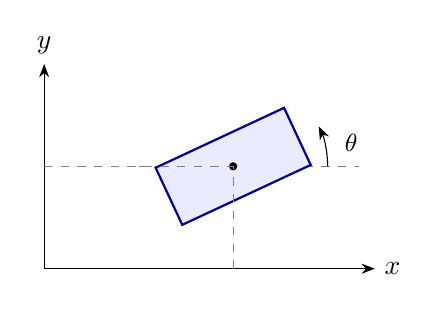
\begin{tikzpicture}[>=Stealth]
  \draw[->] (0,0) -- (4.2,0) node[right] {$x$};
  \draw[->] (0,0) -- (0,2.6) node[above] {$y$};
  \begin{scope}[shift={(2.4,1.3)}]
    \draw[dashed,gray] (-1.2,0) -- (1.6,0);
    \begin{scope}[rotate=25]
      \draw[thick,blue!60!black,fill=blue!8] (-0.9,-0.4) rectangle (0.9,0.4);
    \end{scope}
    \fill (0,0) circle (1.5pt);
    \draw[->] (1.2,0) arc (0:25:1.2);
    \node at (1.5,0.3) {\small $\theta$};
  \end{scope}
  \draw[dashed,gray] (0,1.3) -- (2.4,1.3);
  \draw[dashed,gray] (2.4,0) -- (2.4,1.3);
\end{tikzpicture}
\caption{Polygonal robot in the plane: position of the centre of mass $(x,y)$ and orientation $\theta$.}
\end{figure}

\begin{example}[Polyhedral robot in $\W=\R^3$]
Treat it like the previous case, but add $z$ and two more orientation angles:
\[
  q=(x,y,z,\alpha,\beta,\gamma)^\top,\qquad \C=\R^3\times\SO(3),\qquad n=6.
\]
\end{example}

\begin{definition}[Special Euclidean groups]
The spaces $\R^2\times\SO(2)$ and $\R^3\times\SO(3)$ are called the \emph{special Euclidean groups}, denoted $\SE(2)$ and $\SE(3)$.
\end{definition}

\begin{intuition}
$\SE(n)$ is the set of all rigid motions (a rotation followed by a translation) of $n$-dimensional space. A free rigid body can be moved anywhere and turned any way, so its configuration space is exactly the set of rigid motions: $3$ numbers in the plane ($2$ translations + $1$ rotation), $6$ in space ($3$ translations + $3$ rotations).
\end{intuition}

% =====================================================================
\section{Multi-Body Robots: Manipulators}\pts{4--5}
% =====================================================================

\subsection{Planar manipulator with $n_b$ links}

Consider a planar manipulator with $n_b$ links and $n_b$ (e.g.\ revolute) joints moving in $\W=\R^2$. Each link is a rigid body with 3 degrees of freedom in the plane, so one might expect $3n_b$ generalized coordinates. This is wrong: the links are \emph{connected}, and every joint introduces constraints.

\begin{proposition}[Degrees of freedom of a planar serial arm]
A planar arm of $n_b$ links connected to the ground by $n_b$ revolute joints has
\[
  3n_b-2n_b=n_b
\]
degrees of freedom. Each revolute joint imposes $2$ constraints (the two coordinates of the joint point must coincide on the two bodies it connects).
\end{proposition}

Hence, to describe the configuration we do not need to remember all the constraints: one angle per joint is enough,
\[
  q=\begin{pmatrix}q_1\\q_2\\\vdots\\q_{n_b}\end{pmatrix},\quad n=n_b,\qquad
  \C=\underbrace{\SO(2)\times\dots\times\SO(2)}_{n_b\text{ times}}=\SO(2)^{n_b}.
\]

\begin{figure}[ht]
\centering
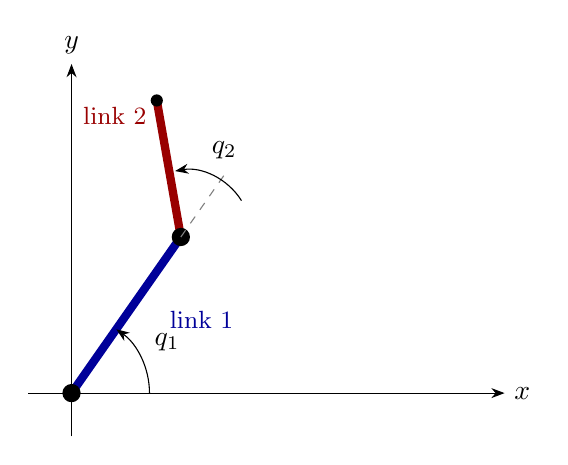
\begin{tikzpicture}[>=Stealth,scale=1.1]
  \draw[->] (-0.5,0) -- (5,0) node[right] {$x$};
  \draw[->] (0,-0.5) -- (0,3.8) node[above] {$y$};
  \coordinate (O) at (0,0);
  \coordinate (J) at (55:2.2);
  \coordinate (E) at ($(J)+(100:1.6)$);
  \draw[line width=3pt,blue!60!black] (O) -- (J);
  \draw[line width=3pt,red!60!black] (J) -- (E);
  \fill (O) circle (3pt);
  \fill (J) circle (3pt);
  \fill (E) circle (2pt);
  \draw[dashed,gray] (J) -- ($(J)+(55:0.9)$);
  \draw[->] (0.9,0) arc (0:55:0.9);
  \node at (28:1.25) {$q_1$};
  \draw[->] ($(J)+(0.7,0.42)$) arc (32:100:0.75) ;
  \node at ($(J)+(0.5,1.0)$) {$q_2$};
  \node[blue!60!black] at (1.5,0.85) {\small link 1};
  \node[red!60!black] at (0.5,3.2) {\small link 2};
\end{tikzpicture}
\caption{A 2R planar arm: one angle per joint is enough to describe the configuration.}
\end{figure}


\begin{figure}[ht]
\centering
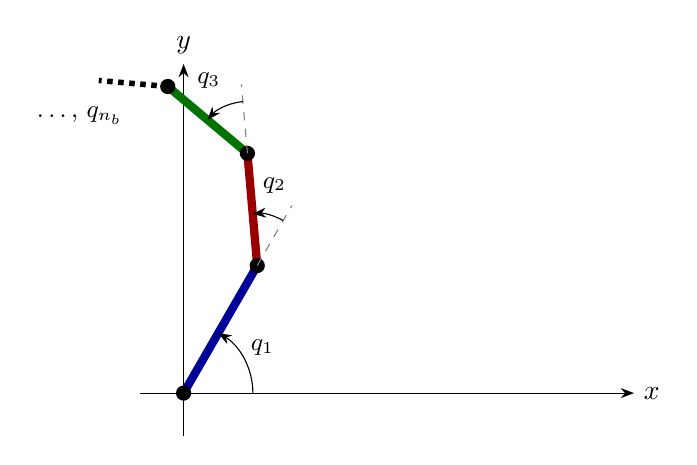
\begin{tikzpicture}[>=Stealth,scale=1.1]
  \draw[->] (-0.5,0) -- (5.2,0) node[right] {$x$};
  \draw[->] (0,-0.5) -- (0,3.8) node[above] {$y$};
  \coordinate (O) at (0,0);
  \coordinate (J1) at (60:1.7);
  \coordinate (J2) at ($(J1)+(95:1.3)$);
  \coordinate (J3) at ($(J2)+(140:1.2)$);
  \draw[line width=3pt,blue!60!black] (O) -- (J1);
  \draw[line width=3pt,red!60!black] (J1) -- (J2);
  \draw[line width=3pt,green!45!black] (J2) -- (J3);
  \draw[line width=2pt,dotted] (J3) -- ($(J3)+(175:0.8)$);
  \foreach \p in {O,J1,J2,J3} \fill (\p) circle (2.5pt);
  % angle arcs
  \draw[->] (0.8,0) arc (0:60:0.8); \node at (30:1.05) {\small $q_1$};
  \draw[dashed,gray] (J1) -- ($(J1)+(60:0.8)$);
  \draw[->] ($(J1)+(60:0.6)$) arc (60:95:0.6); \node at ($(J1)+(78:0.95)$) {\small $q_2$};
  \draw[dashed,gray] (J2) -- ($(J2)+(95:0.8)$);
  \draw[->] ($(J2)+(95:0.6)$) arc (95:140:0.6); \node at ($(J2)+(118:0.95)$) {\small $q_3$};
  \node at (-1.2,3.2) {\small \dots, $q_{n_b}$};
\end{tikzpicture}
\caption{Planar manipulator with $n_b$ links: one joint angle $q_i$ per joint.}
\end{figure}

\begin{intuition}
Imagine gluing the links together at the joints. Each glued joint removes two ``free sliding'' directions. Three links loose in the plane would have $9$ degrees of freedom; pin them into a chain anchored at the base and only $3$ remain: the three joint angles. The number of angles $=$ the number of joints.
\end{intuition}

\begin{proposition}\label{prop:so2-not-so3}
For three revolute joints, $\C=\SO(2)\times\SO(2)\times\SO(2)$, which is very different from $\SO(3)$: the two spaces have the same dimension $3$ but different topology.
\end{proposition}

\begin{intuition}
$\SO(3)$ describes all orientations of \emph{one} rigid body (roll, pitch, yaw). Three planar joints are three \emph{independent} angles each living on its own circle; they cannot all mix into one 3D rotation. Same number of parameters, different shape: it is the shape (topology), not just the count, that matters later.
\end{intuition}

\subsection{Spatial manipulator with $n_b$ links}

\begin{proposition}[Degrees of freedom of a spatial serial arm]
A spatial arm with $n_b$ links and $n_b$ revolute joints in $\W=\R^3$ has
\[
  6n_b-5n_b=n_b
\]
degrees of freedom: each link has $6$ degrees of freedom, but a revolute joint imposes $5$ constraints ($3$ positions and $2$ orientations are fixed; only rotation about the joint axis remains).
\end{proposition}

Even though the manipulator is spatial, each joint has a \emph{planar} orientation (a single angle), so again
\[
  \C=\SO(2)\times\dots\times\SO(2)=\SO(2)^{n_b}\qquad(n_b\text{ times}).
\]

\begin{intuition}
A hinge (revolute joint) always allows exactly one motion: turning about its axis. Whether the world is 2D or 3D, that one motion is a single angle. The ambient dimension changes the \emph{constraint count} ($2$ vs.\ $5$) but not the end result: one angle per joint.
\end{intuition}

% =====================================================================
\section{Topology of $\C$}\label{sec:topology}\pts{5--6}
% =====================================================================

\subsection{The problem with a flat picture of the 2R robot}

Take the 2R planar robot, $\C=\SO(2)\times\SO(2)$, $q=(q_1,q_2)^\top$. Since angles are periodic, $q_1$ and $q_1+2\pi$ give the \emph{same posture}. So if we naively draw $\C$ as the plane $\R^2$ of angle pairs, then two different points give the same posture: the map from this plane to postures is \emph{not injective}, which is bad for us.

\begin{figure}[ht]
\centering
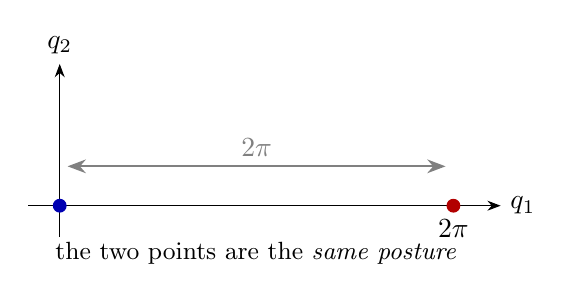
\begin{tikzpicture}[>=Stealth]
  \draw[->] (-0.4,0) -- (5.6,0) node[right] {$q_1$};
  \draw[->] (0,-0.4) -- (0,1.8) node[above] {$q_2$};
  \fill[blue!70!black] (0,0) circle (2.5pt);
  \fill[red!70!black] (5,0) circle (2.5pt);
  \draw[<->,thick,gray] (0.1,0.5) -- (4.9,0.5) node[midway,above] {$2\pi$};
  \node[below] at (5,-0.05) {$2\pi$};
  \node at (2.5,-0.6) {\small the two points are the \emph{same posture}};
\end{tikzpicture}
\caption{On the plane of angle pairs, $q_1=0$ and $q_1=2\pi$ (same $q_2$) correspond to the same posture: the map to postures is many-to-one.}
\end{figure}

A new attempt: restrict each angle to $[0,2\pi)$, i.e.\ draw $\C$ as the square $[0,2\pi)\times[0,2\pi)$. Now the correspondence with postures is one-to-one (considering only the two ``bad sides'' of the square, $q=0$ and $q=2\pi$, as the same). But this is still not good enough: two configurations $q_a$ and $q_b$ that are almost the same posture (one just below $2\pi$, the other just above $0$) look \emph{far apart} in the square.

\begin{figure}[ht]
\centering
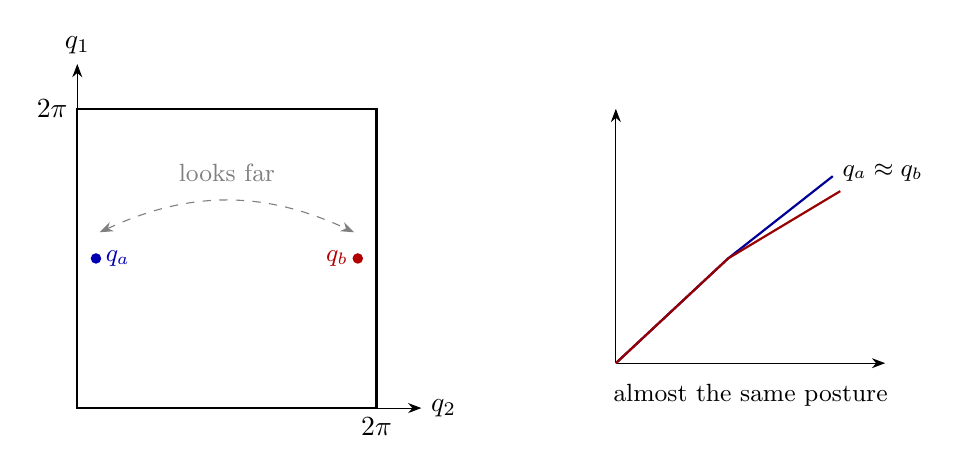
\begin{tikzpicture}[>=Stealth,scale=0.95]
  % square
  \draw[->] (0,0) -- (4.6,0) node[right] {$q_2$};
  \draw[->] (0,0) -- (0,4.6) node[above] {$q_1$};
  \draw[thick] (0,0) rectangle (4,4);
  \node[below] at (4,0) {$2\pi$};
  \node[left] at (0,4) {$2\pi$};
  \fill[blue!70!black] (0.25,2) circle (2pt) node[right] {\small $q_a$};
  \fill[red!70!black]  (3.75,2) circle (2pt) node[left] {\small $q_b$};
  \draw[<->,gray,dashed] (0.3,2.35) to[bend left=25] (3.7,2.35);
  \node[gray] at (2,3.15) {\small looks far};
  % posture plot
  \begin{scope}[shift={(7.2,0.6)}]
    \draw[->] (0,0) -- (3.6,0);
    \draw[->] (0,0) -- (0,3.4);
    \draw[thick,blue!60!black] (0,0) -- (1.5,1.4) -- (2.9,2.5);
    \draw[thick,red!60!black]  (0,0) -- (1.5,1.4) -- (3.0,2.3);
    \node[right] at (2.9,2.55) {\small $q_a\approx q_b$};
    \node[below] at (1.8,-0.15) {\small almost the same posture};
  \end{scope}
\end{tikzpicture}
\caption{The square picture of $\C$: $q_a$ and $q_b$ are close as postures but far in the flat picture.}
\end{figure}

So this topology does not describe exactly what is happening.

\subsection{Wrapping the space: the torus}

The fix is to \emph{wrap} the space: identify the opposite sides of the square (left with right, bottom with top) and embed the resulting 2D object in 3D. We obtain a \emph{torus} (from Latin, ``pillow'').

\begin{figure}[ht]
\centering
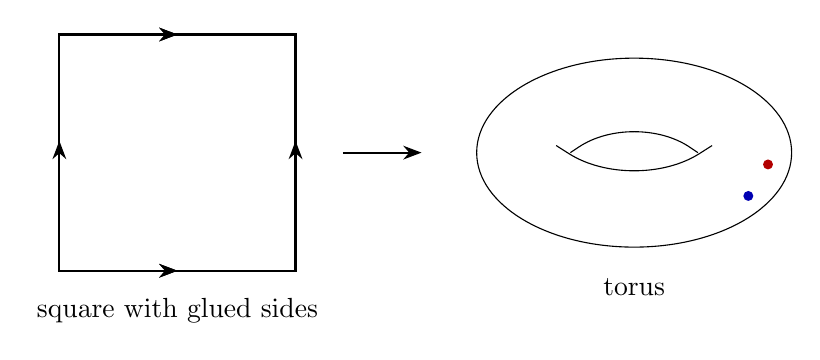
\begin{tikzpicture}[>=Stealth,scale=1]
  % identification square
  \begin{scope}
    \draw[thick] (0,0) rectangle (3,3);
    % vertical sides: single arrow, same direction
    \draw[thick,decoration={markings,mark=at position 0.55 with {\arrow{Stealth}}},postaction={decorate}] (0,0) -- (0,3);
    \draw[thick,decoration={markings,mark=at position 0.55 with {\arrow{Stealth}}},postaction={decorate}] (3,0) -- (3,3);
    % horizontal sides: double arrow
    \draw[thick,decoration={markings,mark=at position 0.5 with {\arrow{Stealth}\arrow{Stealth}}},postaction={decorate}] (0,0) -- (3,0);
    \draw[thick,decoration={markings,mark=at position 0.5 with {\arrow{Stealth}\arrow{Stealth}}},postaction={decorate}] (0,3) -- (3,3);
    \node at (1.5,-0.5) {square with glued sides};
  \end{scope}
  \draw[->,thick] (3.6,1.5) -- (4.6,1.5);
  % torus
  \begin{scope}[shift={(7.3,1.5)}]
    \draw (0,0) ellipse (2 and 1.2);
    \begin{scope}[scale=0.9]
      \path[rounded corners=24pt] (-.9,0)--(0,.6)--(.9,0) (-.9,0)--(0,-.56)--(.9,0);
      \draw[rounded corners=28pt] (-1.1,.1)--(0,-.6)--(1.1,.1);
      \draw[rounded corners=24pt] (-.9,0)--(0,.6)--(.9,0);
    \end{scope}
    \fill[blue!70!black] (1.45,-0.55) circle (1.8pt);
    \fill[red!70!black]  (1.7,-0.15) circle (1.8pt);
    \node at (0,-1.7) {torus};
  \end{scope}
\end{tikzpicture}
\caption{Gluing opposite sides of the square gives a torus. Points that were far apart in the square (across the seam) become neighbours on the torus.}
\end{figure}

\begin{proposition}
$\SO(2)\cong\Sph^1$ (the circle), hence the configuration space of the 2R planar robot is $\Sph^1\times\Sph^1=\mathbb{T}^2$, the torus, and in general $\SO(2)^{n_b}\cong\mathbb{T}^{n_b}$ is an $n_b$-dimensional torus.
\end{proposition}

\begin{intuition}
A joint angle is like a clock hand: after $2\pi$ you are back where you started, so one angle lives on a \emph{circle}, not on a line. Two joints give two circles, and a product of two circles is the surface of a doughnut. Walking off the right side of the square and reappearing on the left is just going around the doughnut the short way.
\end{intuition}

\subsection{Manifolds}

\begin{definition}[Manifold]
A \emph{manifold} of dimension $n$ is a space in which the neighbourhood of each point ``looks like'' a neighbourhood of $\R^n$. (For the torus, $\R^2$.)
\end{definition}

\begin{proposition}
Configuration spaces are manifolds (in general \emph{not} Euclidean anymore): $\R^m$, $\SO(2)$, $\SO(3)$, $\SE(2)$, $\SE(3)$ and their products are all manifolds.
\end{proposition}

\begin{intuition}
The Earth is the classical example: it is a sphere, yet a small enough patch looks flat, so a city map works. Locally we can use ordinary coordinates and calculus; globally the space can wrap around, and that is what a flat picture cannot show.
\end{intuition}

\begin{figure}[ht]
\centering
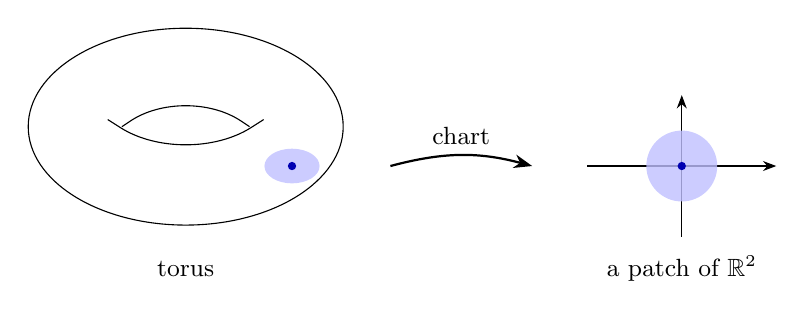
\begin{tikzpicture}[>=Stealth]
  \begin{scope}
    \draw (0,0) ellipse (2 and 1.25);
    \begin{scope}[scale=0.9]
    \path[rounded corners=24pt] (-.9,0)--(0,.6)--(.9,0) (-.9,0)--(0,-.56)--(.9,0);
    \draw[rounded corners=28pt] (-1.1,.1)--(0,-.6)--(1.1,.1);
    \draw[rounded corners=24pt] (-.9,0)--(0,.6)--(.9,0);
    \end{scope}
    \fill[blue!25,opacity=.8] (1.35,-0.5) ellipse (0.35 and 0.22);
    \fill[blue!70!black] (1.35,-0.5) circle (1.5pt);
    \node at (0,-1.8) {\small torus};
  \end{scope}
  \draw[->,thick] (2.6,-0.5) to[bend left=15] node[above] {\small chart} (4.4,-0.5);
  \begin{scope}[shift={(6.3,-0.5)}]
    \draw[->] (-1.2,0) -- (1.2,0);
    \draw[->] (0,-0.9) -- (0,0.9);
    \fill[blue!25,opacity=.8] (0,0) circle (0.45);
    \fill[blue!70!black] (0,0) circle (1.5pt);
    \node at (0,-1.3) {\small a patch of $\R^2$};
  \end{scope}
\end{tikzpicture}
\caption{A small neighbourhood of any point of the torus can be flattened (charted) onto a neighbourhood in $\R^2$: this is what ``looks like $\R^n$'' means.}
\end{figure}

% =====================================================================
\section{Distances in $\C$}\pts{6--8}
% =====================================================================

\subsection{What a distance must satisfy}

\begin{definition}[Distance (metric)]
A function $d:\C\times\C\to\R$ is a \emph{distance} if for all $q_A,q_B,q_C\in\C$:
\begin{enumerate}[nosep,label=(\roman*)]
  \item $d(q_A,q_B)\ge 0$;
  \item $d(q_A,q_B)=0$ if and only if $q_A=q_B$;
  \item $d(q_A,q_B)=d(q_B,q_A)$ (symmetry);
  \item $d(q_A,q_B)\le d(q_A,q_C)+d(q_C,q_B)$ (triangle inequality).
\end{enumerate}
\end{definition}


\begin{figure}[ht]
\centering
\begin{tikzpicture}[>=Stealth]
  \draw[->] (0,0) -- (0,3.2);
  \draw[->] (0,0) -- (3.4,-0.5);
  \draw[->] (0,0) -- (-1.5,-1.2);
  \node at (1.2,3.0) {$\C$};
  \coordinate (A) at (0.6,1.0);
  \coordinate (B) at (2.3,1.6);
  \fill[blue!70!black] (A) circle (2pt) node[left] {$q_A$};
  \fill[red!70!black] (B) circle (2pt) node[right] {$q_B$};
  \draw[green!45!black,very thick] (A) to[bend left=25] node[above] {$d(q_A,q_B)$} (B);
\end{tikzpicture}
\caption{The distance $d(q_A,q_B)$ between two points of the configuration space.}
\end{figure}

\subsection{Distances on manifolds and geodesics}

The classic (Euclidean) distance completely ignores the curvature of the space: for two points on a torus, the straight segment between them passes \emph{through the hole}, outside the manifold. So we cannot use the Euclidean distance.

\begin{figure}[ht]
\centering
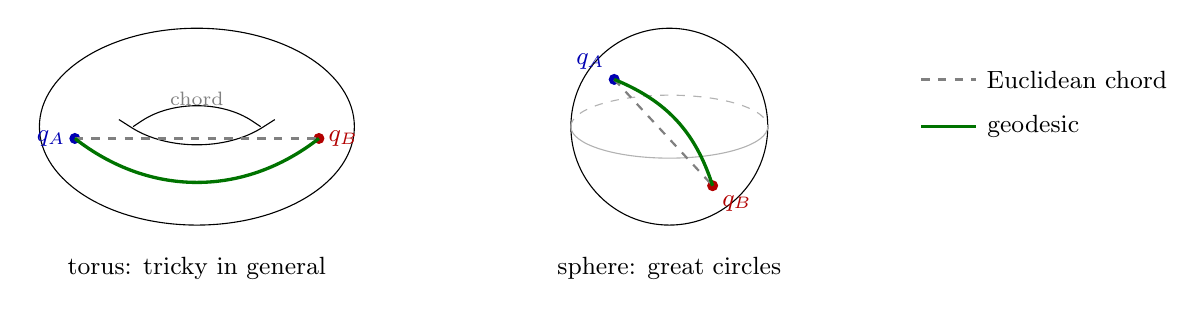
\begin{tikzpicture}[>=Stealth]
  % torus panel
  \begin{scope}
    \draw (0,0) ellipse (2 and 1.25);
    \begin{scope}[scale=0.9]
    \path[rounded corners=24pt] (-.9,0)--(0,.6)--(.9,0) (-.9,0)--(0,-.56)--(.9,0);
    \draw[rounded corners=28pt] (-1.1,.1)--(0,-.6)--(1.1,.1);
    \draw[rounded corners=24pt] (-.9,0)--(0,.6)--(.9,0);
    \end{scope}
    \fill[blue!70!black] (-1.55,-0.15) circle (2pt) node[left] {\small $q_A$};
    \fill[red!70!black]  (1.55,-0.15) circle (2pt) node[right] {\small $q_B$};
    \draw[dashed,gray,thick] (-1.55,-0.15) -- (1.55,-0.15);
    \draw[green!45!black,very thick] (-1.55,-0.15) to[bend right=38] (1.55,-0.15);
    \node at (0,-1.8) {\small torus: tricky in general};
    \node[gray,font=\scriptsize] at (0,0.35) {chord};
  \end{scope}
  % sphere panel
  \begin{scope}[shift={(6,0)}]
    \draw (0,0) circle (1.25);
    \draw[gray!60] (-1.25,0) arc (180:360:1.25 and 0.4);
    \draw[gray!60,dashed] (-1.25,0) arc (180:0:1.25 and 0.4);
    \fill[blue!70!black] (-0.7,0.6) circle (2pt) node[above left] {\small $q_A$};
    \fill[red!70!black]  (0.55,-0.75) circle (2pt) node[below right] {\small $q_B$};
    \draw[dashed,gray,thick] (-0.7,0.6) -- (0.55,-0.75);
    \draw[green!45!black,very thick] (-0.7,0.6) to[bend left=25] (0.55,-0.75);
    \node at (0,-1.8) {\small sphere: great circles};
  \end{scope}
  % legend
  \draw[dashed,gray,thick] (9.2,0.6) -- (9.9,0.6) node[right,black] {\small Euclidean chord};
  \draw[green!45!black,very thick] (9.2,0) -- (9.9,0) node[right,black] {\small geodesic};
\end{tikzpicture}
\caption{The chord between two points leaves the manifold (it crosses the hole of the torus, or the inside of the sphere); the geodesic stays on the surface. On a sphere the geodesic is an arc of a great circle; on a general manifold it is hard to compute.}
\end{figure}

\begin{definition}[Geodesic]
A \emph{geodesic} is a minimum-length path between two points \emph{on the manifold}. The geodesic distance is the length of that path.
\end{definition}

\begin{intuition}
For two cities on Earth, the geodesic is the great-circle route an aircraft follows, not the tunnel through the Earth. Geodesics are the ``honest'' distances on a curved space.
\end{intuition}

\subsection{The displacement metric}

Geodesics are easy on a sphere but can be tricky in general (and on a torus). Because of this difficulty, roboticists do not use them. They use instead a \emph{displacement metric}.

Let $p$ denote a point of the robot (e.g.\ the centre of mass, or the end point of a link), and $p(q)$ its position in $\W$ when the configuration is $q$.

\begin{definition}[Displacement metric]
\[
  d(q_A,q_B)=\max_{p\in\text{robot}}\ \norm{p(q_A)-p(q_B)} .
\]
It is the \emph{maximum displacement} of the points of the robot when moving from $q_A$ to $q_B$.
\end{definition}

\begin{proposition}
The displacement metric satisfies the four axioms of a distance (provided distinct configurations give distinct postures, which is the case for a minimal parametrization).
\end{proposition}

\begin{proof}
(i),(iii) hold because a norm is non-negative and symmetric, and the maximum of such quantities is too. (ii) If $q_A=q_B$ every point has zero displacement, so $d=0$; conversely $d=0$ means every point is at the same place in the two configurations, i.e.\ the postures coincide, hence $q_A=q_B$. (iv) For every point $p$,
\[
 \norm{p(q_A)-p(q_B)}\le\norm{p(q_A)-p(q_C)}+\norm{p(q_C)-p(q_B)}\le d(q_A,q_C)+d(q_C,q_B);
\]
taking the maximum over $p$ on the left gives the claim. \qedhere
\end{proof}

\begin{intuition}
Instead of measuring a length \emph{inside} the curved configuration space, we go back to the physical world and ask: ``how far does the worst-behaved point of the robot have to travel?'' We use ordinary Euclidean distances there, where they are perfectly fine, and the curvature of $\C$ takes care of itself. Nice side effect: this measure is automatically periodic, since $q_1$ and $q_1+2\pi$ give the same positions.
\end{intuition}

\begin{example}[1R robot]
A single link of length $L$ rotating about the origin; $q_A$, $q_B$ are two angles differing by $\Delta\in[0,\pi]$. A point at distance $r\le L$ from the joint moves by the chord $2r\sin(\Delta/2)$, largest at the tip, so
\[
  d(q_A,q_B)=2L\sin\!\big(\tfrac{\Delta}{2}\big).
\]
We are effectively using the \emph{Euclidean} distance between the two tip positions to measure distance on the manifold.
\end{example}

\begin{figure}[ht]
\centering
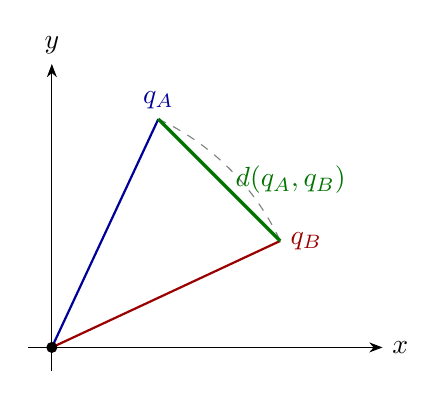
\begin{tikzpicture}[>=Stealth]
  \draw[->] (-0.3,0) -- (4.2,0) node[right] {$x$};
  \draw[->] (0,-0.3) -- (0,3.6) node[above] {$y$};
  \coordinate (O) at (0,0);
  \coordinate (A) at (65:3.2);
  \coordinate (B) at (25:3.2);
  \draw[thick,blue!60!black] (O) -- (A) node[above] {$q_A$};
  \draw[thick,red!60!black] (O) -- (B) node[right] {$q_B$};
  \draw[dashed,gray] (65:3.2) arc (65:25:3.2);
  \draw[very thick,green!45!black] (A) -- (B) node[midway,right=2pt] {$d(q_A,q_B)$};
  \fill (O) circle (2pt);
\end{tikzpicture}
\caption{1R robot: the displacement metric is the Euclidean distance between the tip in the two configurations.}
\end{figure}

\begin{example}[Numbers for the 1R robot, $L=1$]
For $\Delta=\pi/2$: $d=2\sin(\pi/4)=\sqrt2\approx1.41$. For two angles that differ by $2\pi-0.1$ (almost a full turn): the wrapped difference is $0.1$, so $d=2\sin(0.05)\approx0.10$ -- correctly tiny, whereas the flat difference of angles ($6.18$) would call them far apart.
\end{example}

\begin{figure}[ht]
\centering
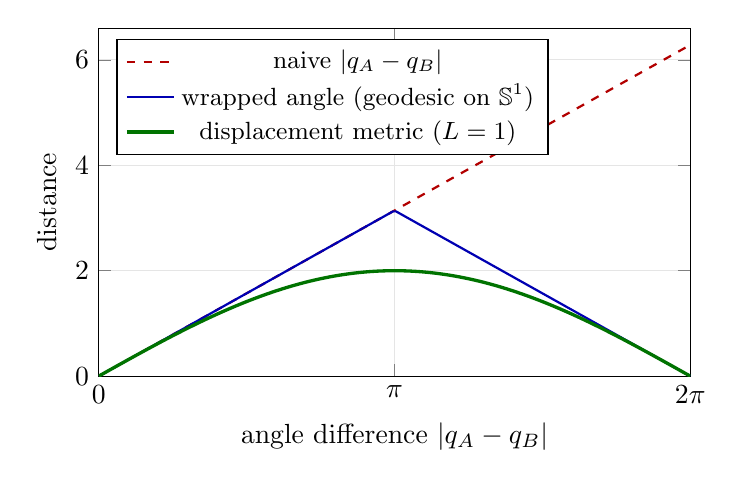
\begin{tikzpicture}
\begin{axis}[width=0.75\linewidth,height=6cm,
  xlabel={angle difference $|q_A-q_B|$},ylabel={distance},
  xmin=0,xmax=2*pi,ymin=0,ymax=6.6,
  xtick={0,pi,2*pi},xticklabels={$0$,$\pi$,$2\pi$},
  trig format plots=rad,legend pos=north west,legend style={font=\small},
  grid=both,grid style={gray!20}]
\addplot[dashed,red!70!black,thick,domain=0:2*pi,samples=100] {x};
\addlegendentry{naive $|q_A-q_B|$}
\addplot[blue!70!black,thick,domain=0:2*pi,samples=200] {min(x,2*pi-x)};
\addlegendentry{wrapped angle (geodesic on $\Sph^1$)}
\addplot[green!45!black,very thick,domain=0:2*pi,samples=200] {2*sin(x/2)};
\addlegendentry{displacement metric ($L=1$)}
\end{axis}
\end{tikzpicture}
\caption{Three ways to measure the distance between two configurations of a 1R robot. The naive difference grows up to $2\pi$; the other two vanish again at $2\pi$ because the configuration wraps around.}
\end{figure}

\begin{example}[2R robot]
With two links we take the maximum over the points of both links. The displacement of a point on a link is an affine function of its position along the link, so its norm is convex and the maximum is attained at a link endpoint: the base (which never moves), the elbow joint, or the tip. In Figure~\ref{fig:2R-disp} (link lengths $1.6$ and $1$) the tip moves by about $0.64$ but the elbow moves by about $1.60$, so $d(q_A,q_B)\approx1.60$: the maximum is \emph{not} necessarily at the tip.
\end{example}

\begin{figure}[ht]
\centering
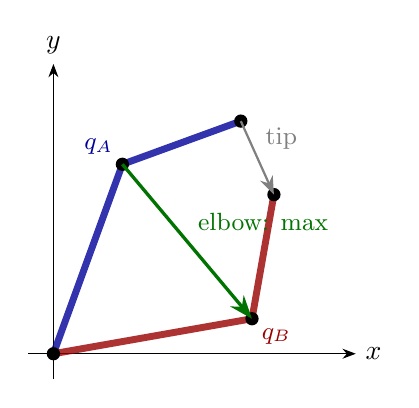
\begin{tikzpicture}[>=Stealth,scale=1.6]
  \draw[->] (-0.2,0) -- (2.4,0) node[right] {$x$};
  \draw[->] (0,-0.2) -- (0,2.3) node[above] {$y$};
  \coordinate (O) at (0,0);
  \coordinate (JA) at (70:1.6);
  \coordinate (EA) at ($(JA)+(20:1)$);
  \coordinate (JB) at (10:1.6);
  \coordinate (EB) at ($(JB)+(80:1)$);
  \draw[line width=2.5pt,blue!60!black,opacity=.8] (O) -- (JA) -- (EA);
  \draw[line width=2.5pt,red!60!black,opacity=.8] (O) -- (JB) -- (EB);
  \fill (O) circle (1.5pt);
  \fill (JA) circle (1.5pt); \fill (EA) circle (1.5pt);
  \fill (JB) circle (1.5pt); \fill (EB) circle (1.5pt);
  \node[blue!60!black,above left] at (JA) {\small $q_A$};
  \node[red!60!black,below right] at (JB) {\small $q_B$};
  \draw[->,very thick,green!45!black] (JA) -- (JB) node[midway,above right] {\small elbow: max};
  \draw[->,thick,gray] (EA) -- (EB) node[midway,above right=-1pt] {\small tip};
\end{tikzpicture}
\caption{2R robot in two configurations. The displacement of each characteristic point is drawn; the displacement metric takes the largest one (here the elbow).}
\label{fig:2R-disp}
\end{figure}

\begin{figure}[ht]
\centering
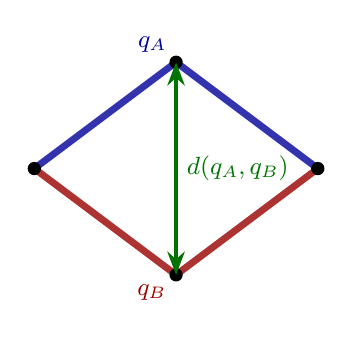
\begin{tikzpicture}[>=Stealth,scale=1.5]
  \coordinate (O) at (0,0);
  \coordinate (E1) at (1.2,0.9);
  \coordinate (E2) at (1.2,-0.9);
  \coordinate (T) at (2.4,0);
  \draw[line width=2.5pt,blue!60!black,opacity=.8] (O) -- (E1) -- (T);
  \draw[line width=2.5pt,red!60!black,opacity=.8] (O) -- (E2) -- (T);
  \foreach \p in {O,E1,E2,T} \fill (\p) circle (1.6pt);
  \draw[<->,very thick,green!45!black] (E1) -- (E2) node[midway,right] {\small $d(q_A,q_B)$};
  \node[blue!60!black,above left] at (E1) {\small $q_A$};
  \node[red!60!black,below left] at (E2) {\small $q_B$};
\end{tikzpicture}
\caption{2R robot with equal links, "elbow up" vs "elbow down", same tip: the tip does not move, and the displacement metric equals the distance between the two elbows.}
\end{figure}

\subsection{The max over infinitely many points}

There is a catch: the definition asks for a maximum over an \emph{infinite} set of points. Intuitively, for polygonal robots we should only look at the \emph{vertices}, but it is not always like this.

\begin{proposition}
If the robot is a convex polygon (or a union of segments, as a chain of links), the maximum in the displacement metric is attained at a vertex (link endpoint).
\end{proposition}

\begin{proof}
Under a rigid motion, the position of a body point $r$ is affine in $r$, so $r\mapsto p(q_A)-p(q_B)$ is affine on the body. The norm of an affine function is convex, and a convex function on a polytope attains its maximum at a vertex.
\end{proof}

\begin{intuition}
The point that moves most is the one sticking out the farthest -- a corner, or the tip of a link. For a curved body (e.g.\ a disk with attached parts) there is no finite list of corners to check, so we need an approximation.
\end{intuition}

\subsection{A practical alternative: control points}

We can use a predetermined number of points, called \emph{control points}, which, if chosen correctly, give a good approximation.

\begin{definition}[Control-point distance]
Fix control points $\{p_1,p_2,\dots,p_c\}$ on the robot. Define
\[
  d(q_A,q_B)=\sum_{i=1}^{c}\norm{p_i(q_A)-p_i(q_B)} .
\]
\end{definition}

\begin{algorithm}[Computing the control-point distance]
\begin{enumerate}[nosep]
  \item Choose $c$ representative points $p_1,\dots,p_c$ on the robot (e.g.\ centre of mass, link endpoints).
  \item For each $i$, compute the forward kinematics $p_i(q_A)$ and $p_i(q_B)$.
  \item Return $\sum_{i=1}^c\norm{p_i(q_A)-p_i(q_B)}$.
\end{enumerate}
\end{algorithm}

\begin{figure}[ht]
\centering
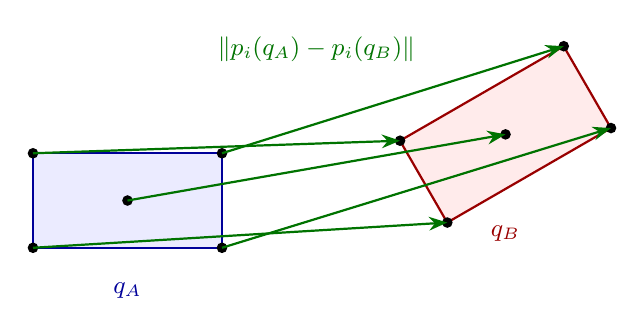
\begin{tikzpicture}[>=Stealth,scale=1.2]
  \begin{scope}[shift={(0,0)}]
    \coordinate (a1) at (-1,-.5); \coordinate (a2) at (1,-.5);
    \coordinate (a3) at (1,.5);   \coordinate (a4) at (-1,.5); \coordinate (a5) at (0,0);
    \draw[thick,blue!60!black,fill=blue!8] (a1) rectangle (a3);
  \end{scope}
  \begin{scope}[shift={(4,0.7)},rotate=30]
    \coordinate (b1) at (-1,-.5); \coordinate (b2) at (1,-.5);
    \coordinate (b3) at (1,.5);   \coordinate (b4) at (-1,.5); \coordinate (b5) at (0,0);
    \draw[thick,red!60!black,fill=red!8] (b1) rectangle (b3);
  \end{scope}
  \foreach \i in {1,2,3,4,5}{
    \fill (a\i) circle (1.6pt);
    \fill (b\i) circle (1.6pt);
    \draw[->,green!45!black,thick] (a\i) -- (b\i);
  }
  \node[blue!60!black] at (0,-0.95) {\small $q_A$};
  \node[red!60!black] at (4,-0.35) {\small $q_B$};
  \node[green!45!black,font=\small] at (2,1.6) {$\norm{p_i(q_A)-p_i(q_B)}$};
\end{tikzpicture}
\caption{Control points $p_1,\dots,p_5$ (four corners and the centre) of a rectangular robot. The distance is the sum of the lengths of the displacement arrows.}
\end{figure}

\begin{proposition}
The control-point distance is symmetric and satisfies the triangle inequality. It is a genuine distance if the control points are chosen so that $p_i(q_A)=p_i(q_B)$ for all $i$ implies $q_A=q_B$; otherwise it is only a pseudo-distance.
\end{proposition}

\begin{proof}
Each summand is a norm of a difference, so symmetry holds, and the triangle inequality holds termwise and is preserved by the sum. The condition on control points gives axiom (ii). 
\end{proof}

\begin{intuition}
Rather than tracking every point, you pin a few ``sensors'' on the robot (say, the tip and the middle) and add up how far they each move. A moving robot cannot fool three well-placed sensors: if they all end up in the same places, the robot is in the same pose. The cost: an approximation of the true worst-case displacement, but cheap and easy to differentiate.
\end{intuition}

% =====================================================================
\section{Summary}
% =====================================================================

\subsection{Configuration spaces seen in this lecture}

\begin{center}
\renewcommand{\arraystretch}{1.25}
\begin{tabular}{@{}llcc@{}}
\toprule
Robot & $\C$ & $n=\dim\C$ & Euclidean? \\
\midrule
Point in $\R^3$ & $\R^3$ & 3 & yes \\
Disk in $\R^2$ & $\R^2$ & 2 & yes \\
Disk with tick / polygon in $\R^2$ & $\SE(2)=\R^2\times\SO(2)$ & 3 & no \\
Polyhedron in $\R^3$ & $\SE(3)=\R^3\times\SO(3)$ & 6 & no \\
Planar $n_b$-R arm & $\SO(2)^{n_b}=\mathbb{T}^{n_b}$ & $n_b$ & no \\
Spatial $n_b$-R arm & $\SO(2)^{n_b}=\mathbb{T}^{n_b}$ & $n_b$ & no \\
\bottomrule
\end{tabular}
\end{center}

\subsection{Distances on $\C$}

\begin{center}
\renewcommand{\arraystretch}{1.25}
\begin{tabular}{@{}p{3.3cm}p{4.2cm}p{4.6cm}@{}}
\toprule
Distance & Definition & Pros / cons \\
\midrule
Euclidean in parameters & $\norm{q_A-q_B}$ & simple, but ignores wrapping (bad on angles) \\
Geodesic & shortest path on the manifold & exact, but hard to compute in general \\
Displacement metric & $\max_p\norm{p(q_A)-p(q_B)}$ & respects topology, physically meaningful; max over infinitely many points \\
Control points & $\sum_i\norm{p_i(q_A)-p_i(q_B)}$ & cheap approximation; needs well-chosen points \\
\bottomrule
\end{tabular}
\end{center}

\subsection{Key take-aways}

\begin{itemize}
  \item The configuration space $\C$ is the space of all values of a \emph{minimal} set of parameters describing the robot; in it the robot is a single point, and planning/control become problems about that point.
  \item Joints reduce degrees of freedom: a planar arm has $3n_b-2n_b=n_b$ and a spatial arm $6n_b-5n_b=n_b$ degrees of freedom -- one angle per joint.
  \item Because angles are periodic, $\C$ is generally a \emph{manifold} (e.g.\ a torus for a 2R arm), not $\R^n$: same dimension does not mean same shape ($\SO(2)^3\ne\SO(3)$).
  \item Euclidean distance in parameter space is misleading on a manifold; geodesics are correct but hard to compute.
  \item Roboticists use the \emph{displacement metric} (max point displacement) or its practical version with a few \emph{control points}.
\end{itemize}

\end{document}